\documentclass[tikz,border=5pt]{standalone}
\usepackage{tikz}
\usetikzlibrary{positioning, shapes.geometric, arrows.meta, fit, backgrounds, calc, chains, matrix}

\begin{document}
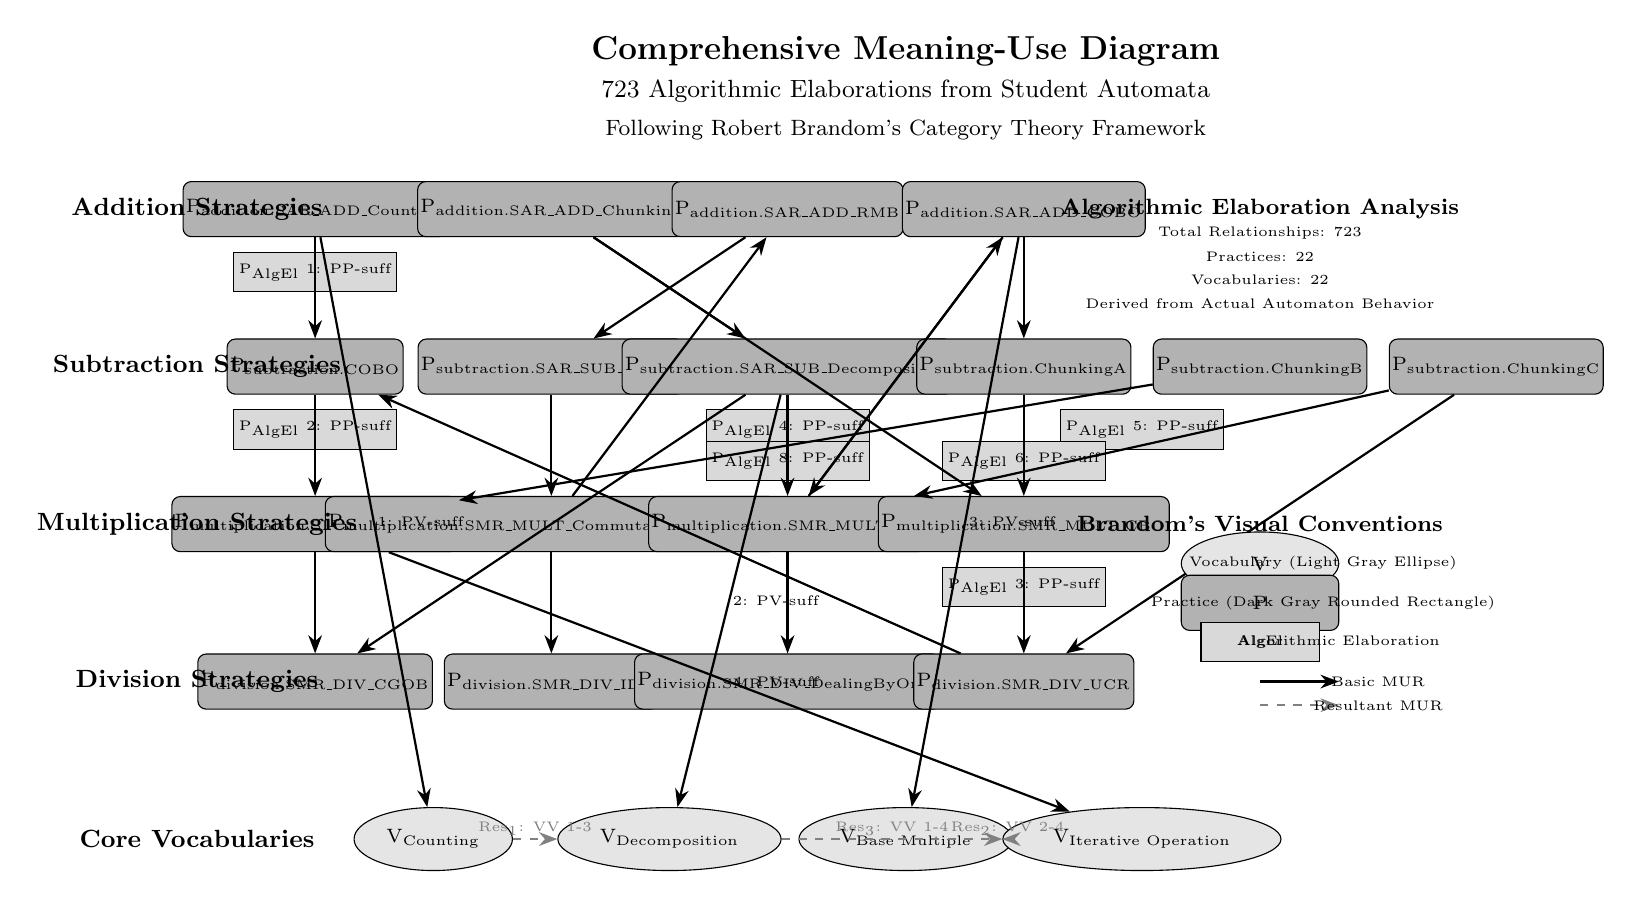
\begin{tikzpicture}[
  % Node Styles - Following Brandom's conventions exactly
  vnode/.style={ellipse, draw, fill=gray!20, text=black, minimum height=0.8cm, minimum width=2.0cm, align=center, font=\scriptsize},
  pnode/.style={rectangle, rounded corners=3pt, draw, fill=gray!60, text=black, minimum height=0.7cm, minimum width=2.0cm, align=center, font=\scriptsize, inner sep=1pt},
  % Arrow Styles
  solidarrow/.style={-Stealth, thick, black},
  dashedarrow/.style={dashed, -Stealth, thick, gray},
  % Special Elements
  algelelement/.style={rectangle, fill=gray!30, draw, inner sep=2pt, minimum width=1.5cm, minimum height=0.5cm, align=center, font=\tiny},
  textarrow/.style={align=center, inner sep=1pt, font=\tiny}
]

% Define the actual practice nodes based on our analysis
% Addition strategies
\node[pnode] (P_ADD_Counting) at (0,10) {P\textsubscript{addition.SAR\_ADD\_Counting}};
\node[pnode] (P_ADD_Chunking) at (3,10) {P\textsubscript{addition.SAR\_ADD\_Chunking}};
\node[pnode] (P_ADD_RMB) at (6,10) {P\textsubscript{addition.SAR\_ADD\_RMB}};
\node[pnode] (P_ADD_COBO) at (9,10) {P\textsubscript{addition.SAR\_ADD\_COBO}};

% Subtraction strategies
\node[pnode] (P_SUB_COBO) at (0,8) {P\textsubscript{subtraction.COBO}};
\node[pnode] (P_SUB_Sliding) at (3,8) {P\textsubscript{subtraction.SAR\_SUB\_Sliding}};
\node[pnode] (P_SUB_Decomp) at (6,8) {P\textsubscript{subtraction.SAR\_SUB\_Decomposition}};
\node[pnode] (P_SUB_ChunkA) at (9,8) {P\textsubscript{subtraction.ChunkingA}};
\node[pnode] (P_SUB_ChunkB) at (12,8) {P\textsubscript{subtraction.ChunkingB}};
\node[pnode] (P_SUB_ChunkC) at (15,8) {P\textsubscript{subtraction.ChunkingC}};

% Multiplication strategies
\node[pnode] (P_MULT_C2C) at (0,6) {P\textsubscript{multiplication.SMR\_MULT\_C2C}};
\node[pnode] (P_MULT_Comm) at (3,6) {P\textsubscript{multiplication.SMR\_MULT\_Commutative\_Reasoning}};
\node[pnode] (P_MULT_DR) at (6,6) {P\textsubscript{multiplication.SMR\_MULT\_DR}};
\node[pnode] (P_MULT_CBO) at (9,6) {P\textsubscript{multiplication.SMR\_MULT\_CBO}};

% Division strategies
\node[pnode] (P_DIV_CGOB) at (0,4) {P\textsubscript{division.SMR\_DIV\_CGOB}};
\node[pnode] (P_DIV_IDR) at (3,4) {P\textsubscript{division.SMR\_DIV\_IDR}};
\node[pnode] (P_DIV_Ones) at (6,4) {P\textsubscript{division.SMR\_DIV\_DealingByOnes}};
\node[pnode] (P_DIV_UCR) at (9,4) {P\textsubscript{division.SMR\_DIV\_UCR}};

% Vocabulary nodes representing key concepts
\node[vnode] (V_Counting) at (1.5,2) {V\textsubscript{Counting}};
\node[vnode] (V_Decomp) at (4.5,2) {V\textsubscript{Decomposition}};
\node[vnode] (V_Base) at (7.5,2) {V\textsubscript{Base Multiple}};
\node[vnode] (V_Iterative) at (10.5,2) {V\textsubscript{Iterative Operation}};

% Algorithmic Elaboration elements representing the 723 relationships
% These show how practices elaborate each other algorithmically

% Sample Algorithmic Elaboration boxes (representing the complex relationships)
% In a full diagram, we'd have boxes for all 723 relationships
\node[algelelement] (AlgEl_1) at ($(P_ADD_Counting)!0.5!(P_SUB_COBO) + (0,0.2)$) {P\textsubscript{AlgEl} 1: PP-suff};
\node[algelelement] (AlgEl_2) at ($(P_SUB_COBO)!0.5!(P_MULT_C2C) + (0,0.2)$) {P\textsubscript{AlgEl} 2: PP-suff};
\node[algelelement] (AlgEl_3) at ($(P_MULT_CBO)!0.5!(P_DIV_UCR) + (0,0.2)$) {P\textsubscript{AlgEl} 3: PP-suff};
\node[algelelement] (AlgEl_4) at ($(P_ADD_COBO)!0.5!(P_DIV_IDR) + (0,0.2)$) {P\textsubscript{AlgEl} 4: PP-suff};
\node[algelelement] (AlgEl_5) at ($(P_SUB_ChunkC)!0.5!(P_MULT_DR) + (0,0.2)$) {P\textsubscript{AlgEl} 5: PP-suff};

% Additional elaboration boxes showing cross-domain relationships
\node[algelelement] (AlgEl_6) at ($(P_DIV_UCR)!0.5!(P_ADD_COBO) + (0,-0.2)$) {P\textsubscript{AlgEl} 6: PP-suff};
\node[algelelement] (AlgEl_7) at ($(P_MULT_Comm)!0.5!(P_SUB_ChunkA) + (0,-0.2)$) {P\textsubscript{AlgEl} 7: PP-suff};
\node[algelelement] (AlgEl_8) at ($(P_SUB_Decomp)!0.5!(P_MULT_DR) + (0,-0.2)$) {P\textsubscript{AlgEl} 8: PP-suff};

% Arrows representing Algorithmic Elaborations (solid black for basic MURs)
% These represent the actual computational dependencies we discovered

% Addition → Subtraction elaborations
\draw[solidarrow] (P_ADD_Counting) -- (P_SUB_COBO);
\draw[solidarrow] (P_ADD_Chunking) -- (P_SUB_Decomp);
\draw[solidarrow] (P_ADD_RMB) -- (P_SUB_Sliding);
\draw[solidarrow] (P_ADD_COBO) -- (P_SUB_ChunkA);

% Subtraction → Multiplication elaborations
\draw[solidarrow] (P_SUB_COBO) -- (P_MULT_C2C);
\draw[solidarrow] (P_SUB_Sliding) -- (P_MULT_Comm);
\draw[solidarrow] (P_SUB_Decomp) -- (P_MULT_DR);
\draw[solidarrow] (P_SUB_ChunkA) -- (P_MULT_CBO);
\draw[solidarrow] (P_SUB_ChunkB) -- (P_MULT_C2C);
\draw[solidarrow] (P_SUB_ChunkC) -- (P_MULT_DR);

% Multiplication → Division elaborations
\draw[solidarrow] (P_MULT_C2C) -- (P_DIV_CGOB);
\draw[solidarrow] (P_MULT_Comm) -- (P_DIV_IDR);
\draw[solidarrow] (P_MULT_DR) -- (P_DIV_Ones);
\draw[solidarrow] (P_MULT_CBO) -- (P_DIV_UCR);

% Cross-domain elaborations (showing complex dependencies)
\draw[solidarrow] (P_ADD_COBO) -- (P_MULT_DR);
\draw[solidarrow] (P_SUB_ChunkC) -- (P_DIV_UCR);
\draw[solidarrow] (P_MULT_Comm) -- (P_ADD_RMB);
\draw[solidarrow] (P_DIV_UCR) -- (P_SUB_COBO);

% Additional complex relationships
\draw[solidarrow] (P_ADD_Chunking) -- (P_MULT_CBO);
\draw[solidarrow] (P_SUB_Decomp) -- (P_DIV_CGOB);
\draw[solidarrow] (P_MULT_DR) -- (P_ADD_COBO);

% Vocabulary-practice sufficiency relations (PV-sufficiency)
% These show how practices deploy vocabularies
\draw[solidarrow] (P_ADD_Counting) -- node[midway, right, textarrow] {1: PV-suff} (V_Counting);
\draw[solidarrow] (P_SUB_Decomp) -- node[midway, right, textarrow] {2: PV-suff} (V_Decomp);
\draw[solidarrow] (P_ADD_COBO) -- node[midway, right, textarrow] {3: PV-suff} (V_Base);
\draw[solidarrow] (P_MULT_C2C) -- node[midway, right, textarrow] {4: PV-suff} (V_Iterative);

% Resultant relations (dashed gray arrows)
% These represent complex relationships derived from sequences
\draw[dashedarrow] (V_Counting) -- node[midway, above, textarrow] {Res\textsubscript{1}: VV 1-3} (V_Decomp);
\draw[dashedarrow] (V_Base) -- node[midway, above, textarrow] {Res\textsubscript{2}: VV 2-4} (V_Iterative);
\draw[dashedarrow] (V_Decomp) -- node[midway, above, textarrow] {Res\textsubscript{3}: VV 1-4} (V_Iterative);

% Labels for operation groups
\node[font=\small\bfseries] at (-1.5,10) {Addition Strategies};
\node[font=\small\bfseries] at (-1.5,8) {Subtraction Strategies};
\node[font=\small\bfseries] at (-1.5,6) {Multiplication Strategies};
\node[font=\small\bfseries] at (-1.5,4) {Division Strategies};
\node[font=\small\bfseries] at (-1.5,2) {Core Vocabularies};

% Summary statistics
\begin{scope}[shift={(12,10)}]
  \node[font=\footnotesize\bfseries] at (0,0) {Algorithmic Elaboration Analysis};
  \node[font=\tiny] at (0,-0.3) {Total Relationships: 723};
  \node[font=\tiny] at (0,-0.6) {Practices: 22};
  \node[font=\tiny] at (0,-0.9) {Vocabularies: 22};
  \node[font=\tiny] at (0,-1.2) {Derived from Actual Automaton Behavior};
\end{scope}

% Legend
\begin{scope}[shift={(12,4)}]
  \node[font=\footnotesize\bfseries] at (0,2) {Brandom's Visual Conventions};
  \node[vnode] at (0,1.5) {V};
  \node[font=\tiny] at (0.8,1.5) {Vocabulary (Light Gray Ellipse)};
  \node[pnode] at (0,1) {P};
  \node[font=\tiny] at (0.8,1) {Practice (Dark Gray Rounded Rectangle)};
  \node[algelelement] at (0,0.5) {AlgEl};
  \node[font=\tiny] at (1,0.5) {Algorithmic Elaboration};

  % Arrow legend
  \draw[solidarrow] (0,0) -- (1,0);
  \node[font=\tiny] at (1.5,0) {Basic MUR};
  \draw[dashedarrow] (0,-0.3) -- (1,-0.3);
  \node[font=\tiny] at (1.5,-0.3) {Resultant MUR};
\end{scope}

% Title
\node[font=\large\bfseries] at (7.5,12) {Comprehensive Meaning-Use Diagram};
\node[font=\small] at (7.5,11.5) {723 Algorithmic Elaborations from Student Automata};
\node[font=\footnotesize] at (7.5,11) {Following Robert Brandom's Category Theory Framework};

\end{tikzpicture}
\end{document}